\documentclass[10pt, a4paper]{article}
\usepackage[paper=a4paper, left=1.5cm, right=1.5cm, bottom=1.5cm, top=3.5cm]{geometry}
\usepackage[T1]{fontenc}
\usepackage[spanish]{babel}
\usepackage[utf8]{inputenc}
\usepackage{indentfirst}
\usepackage{fancyhdr}
\usepackage{a4wide}
\usepackage[dvipsnames,usenames]{color}
\usepackage{float}
\usepackage{amsmath}
\usepackage{listings}
\usepackage{listingsutf8}
\usepackage{graphicx}
\usepackage{amsfonts}
\usepackage{verbatim}
\usepackage{latexsym}
\usepackage{lastpage}
\usepackage[colorlinks=true, linkcolor=blue]{hyperref}
\usepackage{calc}

\newcommand{\f}[1]{\text{#1}}
\newcommand{\real}{\mathbb{R}}
\newcommand{\nat}{\mathbb{N}}
\newcommand{\eme}{\mathcal{M}}
\newcommand{\emeh}{\widehat{\mathcal{M}}}
\newcommand{\ere}{\mathcal{R}}

\sloppy

\setlength{\voffset}{-0.5cm}
\setlength{\hoffset}{0.7cm}
\setlength{\headsep}{0pt}
\setlength{\headheight}{0pt}
\setlength{\oddsidemargin}{-0.7in}
\setlength{\marginparwidth}{-0.5cm}
\setlength{\textwidth}{18cm}
\setlength{\footskip}{2pt}
\setlength{\topmargin}{0in}
\setlength{\textheight}{25cm}
\setlength{\fboxrule}{3pt}

\begin{document}
\thispagestyle{empty}
\begin{center}

\Huge{ \bf{UNIVERSIDAD DE BUENOS AIRES}}
\\
\LARGE{\bf{Facultad de Ciencias Exactas y Naturales}}
\\
\textbf{Departamento de Computaci\'on}
\\
\textbf{Organizaci\'on del Computador}
\vspace{2.0\baselineskip}
\end{center}


\begin{figure}[h] %[h] Aqui [b] para button [t] para top
\begin{center}

\includegraphics[width=100pt]{./image.jpeg}
\end{center}
\end{figure}
\begin{center}
\vspace*{0.7cm}

\huge{\bf TRABAJO PR\'ACTICO N\'UMERO 2}\\
\huge{Nombre de Grupo: Napolitana con Jam\'on y Morrones}
\vspace*{8cm}

\end{center}

\huge{\textbf{Alumnos:}}\\
\\
\vspace*{0.3cm}
\Large{\textsl{Izcovich, Sabrina} $|$ sizcovich@gmail.com $|$ LU 550/11}\\
\vspace*{0.3cm}
\Large{\textsl{L\'opez Veluscek, Matías} \hspace{0.1cm}$|$ milopezv@gmail.com $|$ 926/10}\\
\vspace*{0.3cm}
\vspace{0.5cm}
 
\newpage
%Pagina de titulo e indice
\thispagestyle{empty}
%\large{
\tableofcontents
%}
\newpage
\section{Introducci\'on}
El objetivo de este trabajo pr\'actico fue experimentar utilizando el modelo de programaci\'on SIMD. Para ello, fue requerido implementar seis filtros para procesamiento de im\'agenes (Recortar, Halftone, Umbralizar, Colorizar, Efecto Plasma y Rotar) tanto en $C$ como en $Assembler$.\newline
Por otro lado, debimos analizar la performance de un procesador al hacer uso de las operaciones SIMD. Para ello, realizamos comparaciones de velocidad entre los dos tipos de implementaciones realizados utilizando la herramienta Time Stamp Counter (TSC) del procesador.

\section{Desarrollo}
Nuestro trabajo consistió en implementar los filtros mencionados anteriormente. Para el desarrollo del mismo, diversas herramientas fueron necesarias. En esta sección, se explicita la utilización de las mismas aclarando en qué nos ayudaron a lograr una correcta ejecución de nuestra implementación.  
\subsection{Implementación en C}
En el caso de $C$, las implementaciones se realizaron siguiendo algoritmos sencillos. Para recorrer las matrices de píxeles utilizamos $for$ pues nos pareció lo más conveniente considerando que nuestros valores estaban pre-establecidos y que al colocar un for dentro de otro (uno para las filas y otro para las columnas) era más simple recorrer todas las posiciones de una matriz.\newline
Al probar iterar primero las columnas y luego las filas, rotar.c giraba la imagen hacia el otro lado; luego, nos decidimos por iterar primero las filas y luego las columnas.
\newline
Por otro lado utilizamos, como tipos de datos, enteros y doubles. Esto se debió a que era lo más conveniente para las operaciones que debía realizar nuestro programa ya que el nivel de precisón alcanzado era mayor y esa cualidad es muy importante para no perder información en cada píxel. Un incoveniente que tuvimos y que nos resultó llamativo fue al implementar rotar.c ya que al definir $\sqrt{2}/2$ como double la imagen obtenida presentaba diferencias con la imagen que debíamos encontrar. Para resolverlo, definimos $\sqrt{2}/2$ como float y dicho problema se solucionó.\newline
\newline
Luego, con el fin de disminuir el tiempo de ejecución de los $C$, comprimimos partes del código reduciendo, a su vez, la cantidad de líneas. También, alteramos pequeños detalles que sumados marcarían diferencia. Por ejemplo, cambiamos j++ por ++j.

\subsection{Implementación en Assembler}
En el caso de $Assembler$, utilizamos la extensión SSE para procesar varios bits a la vez. Esta herramienta nos permitió acelerar la ejecución de nuestro programa dado que en cada ciclo (en la mayoría de los casos) fueron tratados 16 bits a la vez.\newline
Nuestros filtros fueron realizados de la siguiente manera:
\begin{itemize}
\item {\textbf{Recortar:}}
En el caso del filtro recortar, procesamos los 4 cuadrantes de la imagen por separado para no confundir las posiciones de origen y destino de los píxeles por lo que la implementación de cada cuadrante resultó ser la misma a diferencia de los offset utilizados.\newline
Dicha implementación consistió, a grandes rasgos, en levantar de a 16 bits desde la posición de origen y pegarlos en la posición de destino. Una vez alcanzado el valor de $tam$, la siguiente fila era procesada.	\newline
Para realizar dicha función no resultó necesario desempaquetar y empaquetar los píxeles pues no debían ser utilizados para realizar cuentas. Por lo tanto, a medida que se los levantaba, se los copiaba tal cual a la imagen destino.\newline
\newline
La función consistió en una seguidilla de los siguientes pasos:\newline
En primer lugar, se procesa el cuadrante B. Para ello, se le resta el $tam$ al ancho de la imagen para obtener el offset. Luego, se calcula el offset vertical de destino multiplicando el dst\_row\_size por tam para continuar ingresando a un ciclo que consiste en mover la porción de memoria del fuente al destino hasta copiar la fila entera del cuadrante. Una vez alcanzado un desplazamiento mayor que el tamaño de la fila, se retrocede la distancia excedida para terminar por procesar el mismo ciclo con los bits que quedaron fuera del pedazo de memoria y debían ser copiados. Dicho procedimiento fue realizado para todas las filas del cuadrante. Para controlar dichos movimientos, fue necesario un contador que nos advirtiera si nos encontrábamos o no en la útlima fila que sería el $tam$.\newline
La misma manipulación fue realizada para el resto de los cuadrantes de manera tal que la imagen quedara de la siguiente forma:\newline

\begin{figure}[H] %[h] Aqui [b] para button [t] para top
\begin{center}
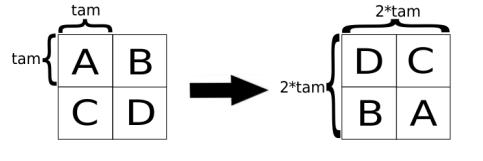
\includegraphics[width=300pt]{./recortar.jpg}
\end{center}
\end{figure}

Luego, comparamos la cantidad de ciclos producidos por $C$ y por $Assembler$.\newline
\begin{itemize}
\item{Comparación de Tiempo}
\end{itemize}
Al probar lena.bmp de 512x512, con una cantidad de 100 iteraciones, el tiempo obtenido fue el siguiente:\newline

Implementación C\newline
----------------\newline

Tiempo de ejecución:\newline
  Comienzo                          : 857860615438390\newline
  Fin                               : 857860685974035\newline
  \# iteraciones                     : 100\newline
  \# de ciclos insumidos totales     : 70535645\newline
  \# de ciclos insumidos por llamada : 705356.500\newline
\newline
Implementación ASM\newline
------------------\newline

Tiempo de ejecución:\newline
  Comienzo                          : 857860758957933\newline
  Fin                               : 857860759960311\newline
  \# iteraciones                     : 100\newline
  \# de ciclos insumidos totales     : 1002378\newline
  \# de ciclos insumidos por llamada : 10023.780\newline
\newline
Resultados\newline
----------\newline

Ciclos C:                 705356.5\newline
Ciclos ASM:               10023.78\newline
Ciclos ASM respecto de C: 1.42109415593\% \newline
Tiempo C:                 70535645\newline
Tiempo ASM:               1002378\newline
Tiempo ASM respecto de C: 1.42109425667\% \newline

\item {\textbf{Halftone:}}
Para la realización de Halftone, debimos guardar en memoria valores que serían necesarios durante la implementación en $Assembler$. Éstos resultaron ser los valores con los que se compararía la sumatoria de los 4 bits como también un inversor (formado por 1's) y distinguidores entre la primer fila y la segunda (formados por 00ff y ff00 consecutivamente).\newline 
Por otro lado, fue necesario que tanto el ancho como el alto de la imagen fueran pares para poder iterar de a dos filas y columnas a la vez. Para ello, dividimos n y m por 2 y comparamos el resto con 0. En caso de serlo, m y n se mantenían. Caso contrario, se le restaba 1 a la variable impar.\newline
Luego, proseguimos recorriendo las matrices de fuente y destino. Para ello, decidimos desplazarnos a través de los punteros, por lo tanto, mientras estuviéramos en la misma fila, nos encargamos de sumarle 16 a rdi y a rsi en cada iteración. Al final de cada ciclo, el valor alcanzado por rsi y rdi era comparado con el ancho-16 para luego decidir si el ciclo debía continuar normalmente o si se había llegado al final de la fila. Una vez que el valor de rdi y rsi llegaban o superaban el ancho-16, se pasaba al final de la fila, donde rdi y rsi se seteaban en el ancho-16 para terminar procesando los últimos 16 bits.\newline
Para procesar los bits, desempaquetamos de a dos filas a word *****. Luego, sumamos los píxeles dos a dos en cada fila. Finalmente, realizamos la suma de las posiciones de las filas correspondientes con las columnas correspondientes de la siguiente manera:\newline
\newline
Considerando la siguiente imagen,
\begin{figure}[H] %[h] Aqui [b] para button [t] para top
\begin{center}
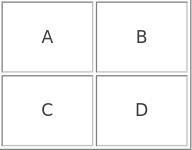
\includegraphics[width=90pt]{./suma.jpg}
\end{center}
\end{figure}
los pasos realizados fueron:\newline
- A+B\newline
- C+D\newline
- (A+B) + (C+D)\newline

Luego, se prosiguió realizando la comparación pcmpgtw entre la suma y los valores seteados para la comparación. Dado que el resultado deseado era el inverso ($\leq$ en vez de $>$), se aplicó un xor con el inversor explicitado anteriormente a cada resultado obtenido por la comparación. Por último, se realizó un and entre lo obtenido de invertir la comparación y los filtrados de primera y segunda fila. Esta suma de operaciones debieron realizarse la cantidad de veces necesaria para cubrir todos los valores con los que comparar la suma de píxeles. Luego, 4 veces. Por último, las máscaras fueron unidas con un 'or' en el que se juntaron la primera con su respectiva segunda fila de cada columna. Los píxeles resultantes fueron, entonces, ubicados en la matriz destino.\newline
Los píxeles resultantes debían cumplir con la siguiente condición:
\begin{figure}[H] %[h] Aqui [b] para button [t] para top
\begin{center}
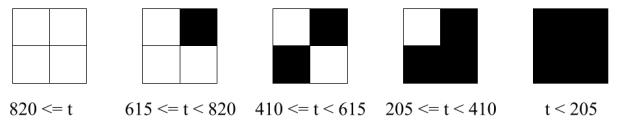
\includegraphics[width=400pt]{./halftone.jpg}
\end{center}
\end{figure}
Por último, utilizamos un registro que era seteado en 1 una vez que se llegaba a la última columna para dar lugar al pasaje de fila y, recorrer de esta manera, la matriz entera.

\begin{itemize}
\item{Comparación de Tiempo}
\end{itemize}
Al probar lena.bmp de 512x512, con una cantidad de 100 iteraciones, el tiempo obtenido fue el siguiente:\newline


\item {\textbf{Umbralizar:}}
En Umbralizar, la imagen destino debía cumplir los siguientes requisitos:
- Cada píxel menor a $min$ debía valer 0.\newline
- Cada píxel mayor a $max$ debía valer 255.\newline
- Caso contrario, el píxel debía valer $\lfloor p/Q \rfloor$.Q\newline
con $min$, $max$ y $Q$ enteros de 1 byte.\newline
Para lograr esto, pasamos dichos valores enteros a floats para realizar los cálculos necesarios habiendo desempaquetado y convertido los píxeles al mismo tipo de dato.\newline
Nuestro ciclo consistió en procesar de a 16 bits comparando los píxeles con $max$ y $min$ con la operación pcmpgtw. Las máscaras resultantes fueron luego invertidas dado que el resultado deseado era la comparación inversa a la facilitada por Intel. Luego, se debieron procesar los píxeles que no fueron menores a $min$ ni mayores a $max$.  
\begin{itemize}
\item{Comparación de Tiempo}
\end{itemize}
Al probar lena.bmp de 512x512, con una cantidad de 100 iteraciones y 64 128 16 como parámetros, el tiempo obtenido fue el siguiente: \newline

Implementación C\newline
----------------\newline

Tiempo de ejecución:\newline
  Comienzo                          : 857572172822622\newline
  Fin                               : 857572676855448\newline
  \# iteraciones                     : 100\newline
  \# de ciclos insumidos totales     : 504032826\newline
  \# de ciclos insumidos por llamada : 5040328.500\newline
\newline
Implementación ASM\newline
------------------\newline

Tiempo de ejecución:\newline
  Comienzo                          : 857572838473791\newline
  Fin                               : 857572938386751\newline
  \# iteraciones                     : 100\newline
  \# de ciclos insumidos totales     : 99912960\newline
  \# de ciclos insumidos por llamada : 999129.625\newline
\newline
Resultados\newline
----------\newline

Ciclos C:                 5040328.5\newline
Ciclos ASM:               999129.625\newline
Ciclos ASM respecto de C: 19.8227084802\%\newline
Tiempo C:                 504032826\newline
Tiempo ASM:               99912960\newline
Tiempo ASM respecto de C: 19.8227089281\%\newline

\item {\textbf{Colorizar:}} 
\begin{itemize}
\item{Comparación de Tiempo}
\end{itemize}
Al probar lena.bmp de 512x512, con una cantidad de 100 iteraciones y 64 128 16 como parámetros, el tiempo obtenido fue el siguiente:\newline
\item {\textbf{Waves:}}

\begin{itemize}
\item{Comparación de Tiempo}
\end{itemize}
Al probar lena.bmp de 512x512, con una cantidad de 100 iteraciones y 2.0 4.0 16.0 como parámetros, el tiempo obtenido fue el siguiente:\newline

Implementación C\newline
----------------\newline

Tiempo de ejecución:\newline
  Comienzo                          : 858182624211702\newline
  Fin                               : 858224537429979\newline
  \# iteraciones                     : 100\newline
  \# de ciclos insumidos totales     : 41913218277\newline
  \# de ciclos insumidos por llamada : 419132160.000\newline
\newline
Implementación ASM\newline
------------------\newline

Tiempo de ejecución:\newline
  Comienzo                          : 858224711685883\newline
  Fin                               : 858225286387416\newline
  \# iteraciones                     : 100\newline
  \# de ciclos insumidos totales     : 574701533\newline
  \# de ciclos insumidos por llamada : 5747015.000\newline
\newline
Resultados\newline
----------\newline
Ciclos C:                 419132160.0\newline
Ciclos ASM:               5747015.0\newline
Ciclos ASM respecto de C: 1.37117013402\%\newline
Tiempo C:                 41913218277\newline
Tiempo ASM:               574701533\newline
Tiempo ASM respecto de C: 1.37117013826\%\newline

\item {\textbf{Rotar:}} 

\begin{itemize}
\item{Comparación de Tiempo}
\end{itemize}
Al probar lena.bmp de 512x512, con una cantidad de 100 iteraciones, el tiempo obtenido fue el siguiente:\newline
Implementación C\newline
----------------\newline

Tiempo de ejecución:\newline
  Comienzo                          : 858387565588994\newline
  Fin                               : 858388404276534\newline
  \# iteraciones                     : 100\newline
  \# de ciclos insumidos totales     : 838687540\newline
  \# de ciclos insumidos por llamada : 8386875.500\newline
\newline
Implementación ASM\newline
------------------\newline

Tiempo de ejecución:\newline
  Comienzo                          : 858388558871397\newline
  Fin                               : 858388874991387\newline
  \# iteraciones                     : 100\newline
  \# de ciclos insumidos totales     : 316119990\newline
  \# de ciclos insumidos por llamada : 3161200.000\newline
\newline
Resultados\newline
----------\newline

Ciclos C:                 8386875.5\newline
Ciclos ASM:               3161200.0\newline
Ciclos ASM respecto de C: 37.6922251916\%\newline
Tiempo C:                 838687540\newline
Tiempo ASM:               316119990\newline
Tiempo ASM respecto de C: 37.6922244487\%\newline


\end{itemize}

hay que poner el pseudocodigo detallado que utilizamos explicando por que recorrimos de la manera que recorrimos la matriz y por que nos parecio lo mas efectivo y eficiente para programar, detallando para que sirve cada cosa. Tambien tenemos que decir que cosas hicimos para facilitar la implementacion en asm, o sea si lo hicimos pensando en como ibamos a resolverlo en asm o si directamente lo hicimos de una manera que fuera rapida. algo que se me ocurre es que preferimos, por ejemplo, usar muchas variables para definir pequeñas operaciones que usaba una sola ecuacion en vez de que fuera todo resuelto de una para poder darles tipos a esas operaciones y que el resultado fuera mas preciso y acertado a lo pedido.\newline

que transformaciones podriamos hacer para que sea mejor lo que hacemos, mejor tiempo, que fue lo que probamos, etc. Por ejemplo si paso de float a double. En umbralizar pasamos Q de float a double. Pusimos Q, max y min en double porque para hacer las cuentas con doubles era lo mas conveniente.
\newline
\section{Resultados}

A partir de los resultados otorgados por un script realizado para calcular el tiempo de ejecución de cada función en $C$ y $Assembler$, decidimos utilizar objdump para lograr dar una explicación a lo obtenido:\newline
En primera instancia, hallamos que la cantidad de ciclos realizados por $Assembler$ es muy menor a la realizada por $C$. Esto se debe a que el $Assembler$ de $C$ realiza múltiples llamados a memoria en cada ciclo. Por ejemplo, la mayoría de los datos que utiliza son almacenados en la pila por lo que en cada iteración realiza operaciones utilizando, por ejemplo, [rbp-0x28]. Esta es la causa principal del retraso temporal generado por el $C$ respecto del $Assembler$. \newline 
Por otro lado, nos resultó sorprendente la extensión de los códigos en $Assembler$ generados por los $C$ en comparación con los nuestros. Para hallarle una explicación a dicha consecuencia, pensamos que el causante de esto fue que, al estar todo almacenado en la pila, los desplazamientos requieren de numerosas instrucciones. Contrariamente, al moverse con un puntero, lo único necesario para el desplazamiento no es más que un sumador. \newline
Por otra parte, hallamos que los códigos en $Assembler$ generados por los $C$ realizan operaciones innecesarias, como por ejemplo multiplicar por 1, dado que se producen de manera automática.\newline
Por último, encontramos que el ensamblado del $C$ no realiza empaquetamientos por lo que la cantidad de operaciones a realizar está multiplicada por 16.\newline

tenemos que hacer un grafico, creo que podriamos hacer uno que para cada funcion que hicimos ponga el tiempo que tardo en asm y en .c y que una por un lado todos los .c y por el otro todos los .asm cuestion de ver precisamente cual es la relacion entre la velocidad de un asm y de un .c. tambien tenemos que hacer uno que muestre graficamente el contenido de los xmm a medida que avanza la ejecucion del programa\newline
aca hay que poner tablas y graficos con los resultados. analizar y comparar las implementaciones. podriamos ejecutar el timing en distintas computadoras y ver que cambia respecto del procesador usado.
\section{Conclusi\'on}
Podemos concluir que las causas principales de que el código en $C$ sea mucho más lento que el código $Assembler$ dado que su ensamblado no utiliza empaquetamiento y almacena todos los datos en la pila que son llamados en cada iteración. Esto significa que $C$ usa la FPU que es poco performante causando un aumento del tiempo de ejecución.\newline
A partir de aquí, podemos concluir que realizar operaciones empaquetando y desempaquetando los datos acelera enormemente la ejecución de una función como también evitar los llamados a memoria dentro de los ciclos.

\end{document}
